\section{Эксперименты}
\label{sec:Chapter4} \index{Chapter4}

\begin{figure}
\centering
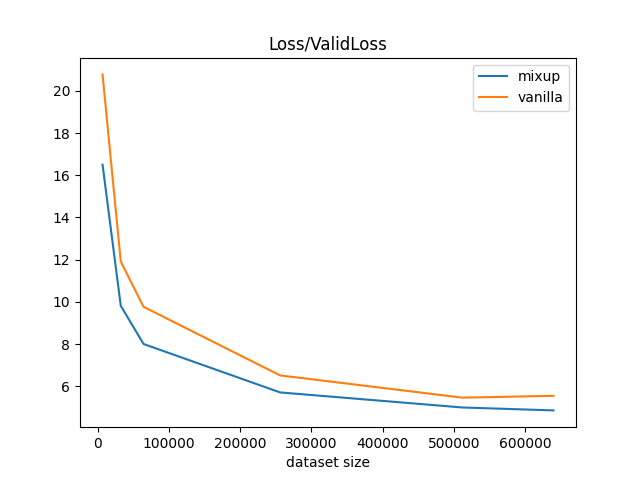
\includegraphics[scale=0.75]{./images/mixup_size/all/ValidLoss.png}
\caption{\protect\hypertarget{image13}{Падение функции ошибки \\ при росте размера датасета (в количестве образцов)}.}
\end{figure}

\subsection{Влияние положения Mixup}
Рассматривались положения mixup между FeatureBlock-ами, а также между последними двумя ConvBN. Точнее говоря, если описывать псевдокодом модель ResNet, рассматриваемые точки для mixup выглядят следующим образом:

\begin{lstlisting}
for i in range(5):
    x = mixup(x)                    # before_block_i
    x = self.blocks[i](x)

x = mixup(x)                        # after_blocks
x = self.final_conv1(x)
x = mixup(x)                        # after_final_conv1
x = self.final_conv2(x)
x = self.final_drop(x)
\end{lstlisting}

Основываясь на результатах \hyperlink{cite.Bas19}{[16]}, были проанализированы все варианты набора позиций для mixup, подходящие под следующие условия:
\begin{enumerate}
\item В каждом наборе присутствуют лишь 2 или 3 точки, где происходит mixup.
\item Позиции в наборе не идут последовательно друг за другом в порядке операций.
\end{enumerate}

Каждый набор позиций был проверен на части датасета размером в $N = 128'000$ образцов \hyperref[tab:mixup_position]{[Таблица 5]}. Как по всем метрикам, так и по функции ошибки, набор before-block0;before-block3 оказался наилучшим \hyperref[tab:mixup_position]{[Таблица 5]}. Далее, если не сказано иного, в качестве набора позиций для mixup везде берется before-block0;before-block3.

Выбор количества точек обусловлен результатами \hyperlink{cite.Bas19}{[16]}. По функции ошибки и всем метрикам на втором месте находится набор из 3 точек для mixup. Улучшение всех метрик и функции ошибки происходит при любом из рассмотренных наборов. Тем не менее, выбор набора важен и влияет на ход обучения.

\newpage
\subsection{Зависимость от количества данных}

\begin{table}[]
\centering
\begin{tabular}{||c c c c c||} 
 \hline
 type & ValidLoss & CharAcc & FragAcc & WordAcc \\ [0.5ex] 
 \hline\hline
 vanilla & 5.55 & 87.56 & 56.28 & 59.93\\ 
 \hline
 mixup & 4.85 & 88.05 & 56.87 & 60.93\\ [1ex] 
 \hline
\end{tabular}
\caption{Функция ошибки и метрики при $N = 640'000$ образцах}
\label{tab:mixup_size_max}
\end{table}

\begin{figure}
\centering
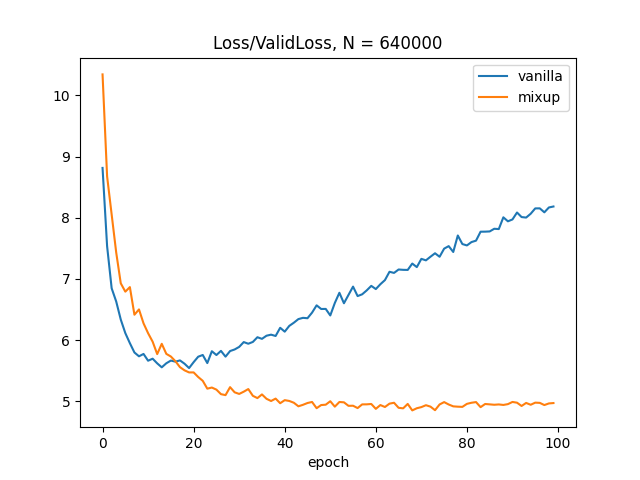
\includegraphics[scale=0.5]{./images/mixup_size/10000_ValidLoss.png}
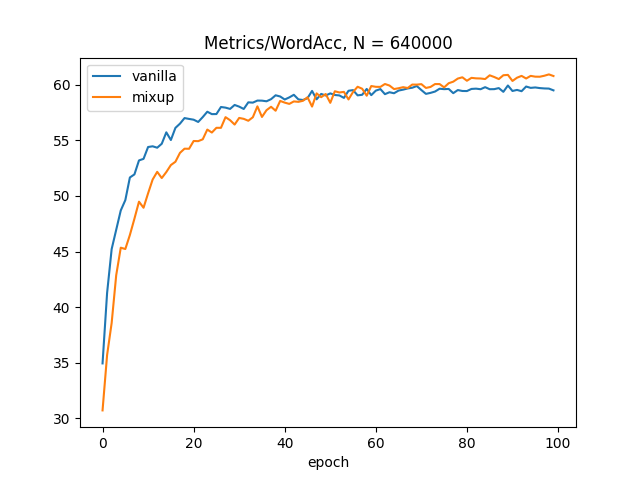
\includegraphics[scale=0.5]{./images/mixup_size/10000_WordAcc.png}
\caption{\protect\hypertarget{image14}{Функция ошибки и метрики при $N = 640'000$ образцах}.}
\end{figure}


Исследовалась зависимость вклада mixup на обучение от количества данных. Эксперименты проводились со следующими размерами датасетов (в образцах):\\ $6400, 32000, 64000, 256000, 512000, 640000$.

Согласно результатам \hyperref[tab:mixup_size_max]{[Таблица 1]} \hyperref[tab:mixup_size]{[Таблица 2]} \hyperref[tab:mixup_size_all]{[Таблица 3]} \hyperref[tab:mixup_size_main]{[Таблица 4]}, mixup улучшает все метрики на любом количестве данных. Более того, mixup хорошо препятствует переобучению \hyperref[tab:mixup_size]{[Таблица 2]}. В частности, функция ошибки на валидационном наборе имеет тенденцию увеличиваться в какой-то момент без использования mixup, в то время как при mixup она достигает некоторой горизонтальной асимптоты \hyperlink{image13}{[Рис 13.]}. Это подтверждает, что mixup оказывает некоторый эффект регуляризации на сеть, как упоминалось ранее.

Также оказалось, что mixup замедляет процесс обучения на начальных эпохах. Интересно, что это замедление длится все дольше при увеличении объема датасета. Например, при N = 640'000 функция ошибки при использовании mixup становится меньше только начиная с $\sim 20$ эпохи, в то время как для метрику WordAcc mixup улучшает только к $\sim 50$ эпохе. Это видно на \hyperlink{image14}{[Рис 14.]}.
\newpage
